\documentclass{beamer}
\usepackage{tikz}
\usetikzlibrary{shapes,arrows}

\usepackage{verbatim}
\usepackage[active,tightpage]{preview}
\PreviewEnvironment{tikzpicture}
\setlength\PreviewBorder{5pt}%
%%%>
\usetikzlibrary{positioning}

\newcommand{\yslant}{0.5}
\newcommand{\xslant}{-0.6}
\tikzset{
	invisible/.style={opacity=0},
	visible on/.style={alt={#1{}{invisible}}},
	alt/.code args={<#1>#2#3}{%
		\alt<#1>{\pgfkeysalso{#2}}{\pgfkeysalso{#3}} % \pgfkeysalso doesn't change the path
	},
}


\begin{document}
	
	\begin{frame}

	% Define block styles
	\tikzstyle{decision} = [diamond, draw, fill=blue!20, 
	text width=4.5em, text badly centered, node distance=5cm, inner sep=0pt]
	\tikzstyle{block} = [rectangle, draw, fill=white, 
	text width=5em, text centered, rounded corners, minimum height=4em]
	\tikzstyle{line} = [draw, -latex']
	\tikzstyle{cloud} = [draw, ellipse,red!80, node distance=5cm,
	minimum height=2em]

	\begin{tikzpicture}[scale=0.8, every node/.style={scale=0.7},node distance = 5cm, auto]
				 \only<2->
				 {
 				\node [decision ] (decide) {Peut-il être stocké sur une machine ?};
 				}
 			
				\node [cloud,fill=white,left of=decide] (g) {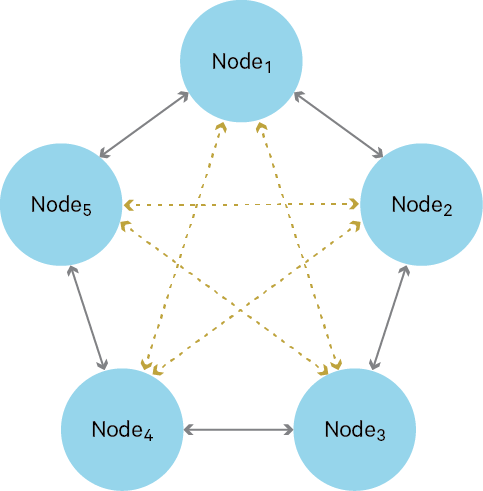
\includegraphics[width=1.5cm]{petri}};

				\only<3->
				{
					\node [block, below of=decide] (stockable) {
\includegraphics[width=1.5cm]{pc}};
				}
				\only<7->
				{
				\node [block, right of=decide,text width=10em, blue] (distribution)  {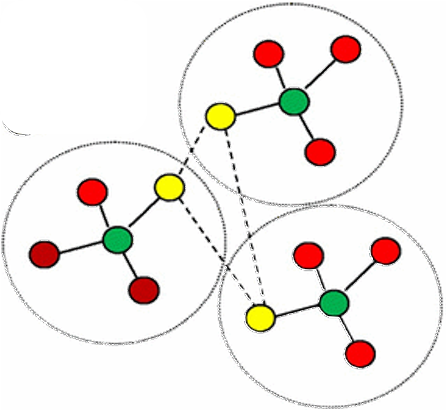
\includegraphics[width=3cm]{graphD}};
				}
				\only<5->
				{	
				\node [decision,below of=stockable] (tempsR) {Temps de reponse rainsonnable ?};
				}
				\only<6->
				{
					\node [block,below of=tempsR,blue ] (m) {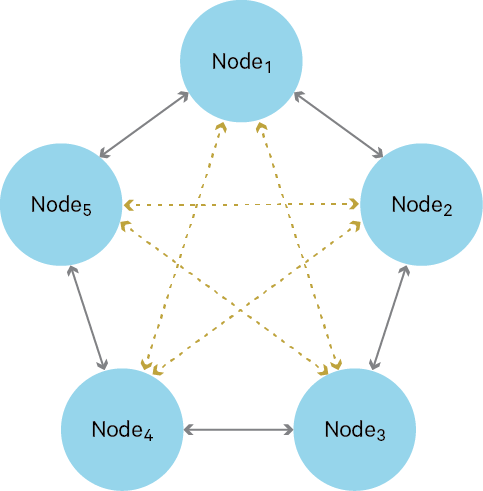
\includegraphics[width=2cm]{petri}};
				}
			\only<9->			
			{
				\node [block, right of=distribution,text width=10em ] (cdistribuer) {Comment Distribué ?}; 
			}
			% Draw edges
 			\path [line,visible on=<2-> ] (g) -- (decide);
			\path [line,visible on=<3-> ] (decide) --node {OUI} (stockable);
 			\path [line,visible on=<8-> ] (decide) -- node {NON}(distribution);
		 	\path [line,visible on=<5-> ] (stockable) --(tempsR);
		 	\path [line,visible on=<6-> ] (tempsR) -- node {OUI}(m);
		 	\path [line,visible on=<7-> ] (tempsR) -| node [near start] {NON}(distribution);
		 	\path [line,visible on=<9-> ] (distribution) -- (cdistribuer);
 
	\end{tikzpicture}
	\end{frame}
 
\end{document}